\section{Advantages}
Logistic regression with a polynomial hypothesis is often way to expensive. This is because each feature space has to be compared to each other, which leads to way too many input features to optimize.

\section{Artificial Neuron}
\begin{itemize}
    \item Feed input via input nodes
    \item Logistic unit does some computation
    \item Sends output
\end{itemize}

\bigskip
\begin{figure}[H]
\centering
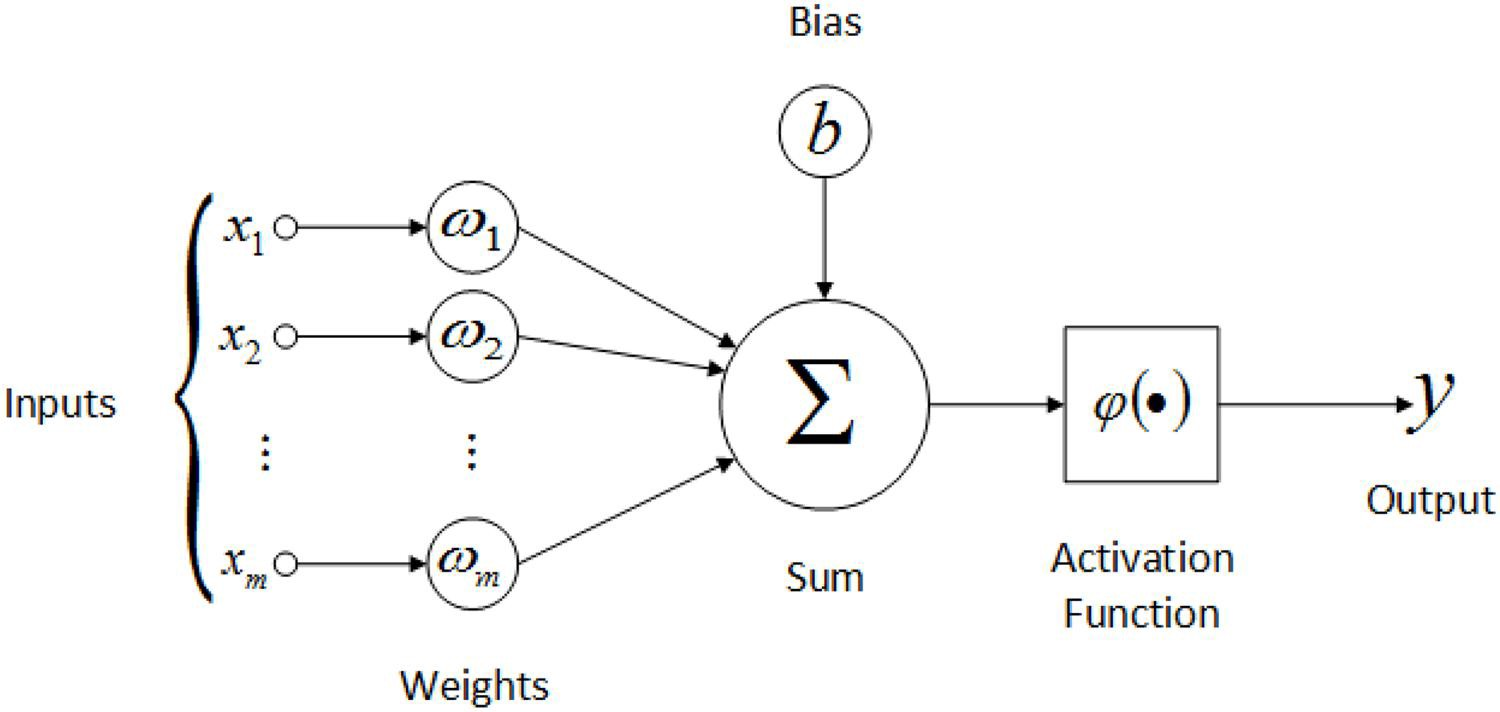
\includegraphics[scale=0.25]{figures/artificialneuron.jpeg}
\caption{Artificial Neuron}
\end{figure}

The activation function is typically the sigmoid function, a hyperbolic tangent, or a rectified linear unit (ReLU).

\section{Notations}
\begin{itemize}
    \item $a_i^{(j)}$ - Activation of unit $i$ in layer $j$ (the output of the node)
    \item $\theta^{(j)}$ - Matrix of parameters (controlling the activation from one layer to the next)
    \item $g(\theta^Tx)$ - The activation function
\end{itemize}

\section{Multiclass Classification}
\begin{itemize}
    \item Given $N$ classes:
    \begin{itemize}
        \item Build a neural network with $N$ output units
        \item Use one-hot encoding to encode the output as an array of $N-1$ zeros and one $1$.
    \end{itemize}
\end{itemize}

\section{Cost function for Neural Networks}
The cost function can generate $k$ outputs, meaning that the sigmoid function (or any other cost functions) returns a $k$ dimensional vector.

The cost function is combined by two parts.

\bigskip

The first part finds the mean of the sum of each training sample $m$, over the sum of each class $k$. All classes has a "one-vs-all" comparison. This gives the following expression:

\[
    -\frac{1}{m}\left[\sum_{i=1}^m\sum_{k=1}^Ky_k^{(i)} \log\left(h_\Theta(x^{(i)})\right)_k+(1-y_k^{(i)}) \log\left(1-(h_\Theta(x^{(i)}))_k\right)\right]
\]

The second part is the regularization term. In this part, we sum all layers $L-1$, over all units in each layer $s_t$, over all the input layers $j$:

\[
    \frac{\lambda}{2m}\sum_{l=1}^{L-1}\sum_{i=1}^{s_t}\sum_{j=1}^{s_l+1}(\Theta_{ji}^{(l)})^2
\]

\section{Learn this better...}

% 31.30

% \bigskip
% \begin{figure}[H]
% \centering
% \includegraphics[scale=0.5]{figures/}
% \caption{}
% \end{figure}

% \begin{theo}[]{theo:theo}
% \label{eq:}
% \[
% a
% \]
% \end{theo}
%
% \section{}